%travail_observator
\subsection{Observateur}
\begin{figure}[h]
\begin{center}
    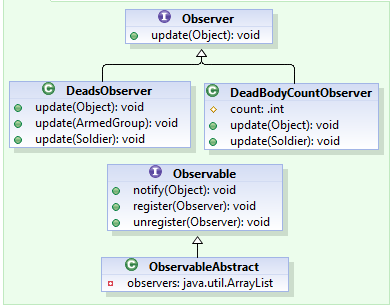
\includegraphics[width=11cm]{diagClassObserver}
\end{center}
    \caption{Diagramme de classes du pattern observeur}
    \label{classes-oberveur}
\end{figure}

Une des problématiques de ce projet était de pouvoir suivre le déroulement des conflits au fur et à mesure du déroulement de l’action. Nous aurions pu produire de nombreux print dans nos fonctions, ce qui aurait généré des affichages au fur et à mesure du déroulement des batailles. Cependant, cette méthode est peu flexible et peu maintenable ! 
C'est donc ici que le pattern \emph{Observateur} va être intéressant, car il nous permet d'observer un objet et d'être notifié de ses changements afin d'appliquer les traitements adéquats suite à ces changements. 
Ainsi, pour afficher au fur et à mesure les noms des soldats morts au sein d'un groupe armé ainsi que les armés détruites, nous avons mis en place le système visible en figure \vref{classes-oberveur}. Il est composé en premier lieu d'une interface \emph{Observer} avec pour sous-classe \emph{DeadsObserver}. Cette dernière se chargera de réaliser l'affichage. Nous avons également rendu observable notre classe \emph{ArmedGroup} en créant l'interface \emph{Observable}. \emph{ObservableAbstract} implémente cette interface et contient une liste d'\emph{Observers}, liste qui permet à l'objet, lorsqu'il change, d'en informer tous ses observateurs. 
Cette classe est également intéressante car elle permet de définir une interdépendance de type un à plusieurs, de tel façon que si on souhaite envoyer des télégrammes d’excuse à une liste d'ami une fois qu'un soldat meurt, on pourra notifier tous les objets qui dépendent du mort. L'inconvénient et la limite du pattern est que le graphe des relations d'observation peut vite devenir complexe. En effet, si l'on veut mettre en place le système des envoi de télégrammes d’excuse à ses amis, il va falloir que chaque objet soit observé par tous les autres objets « amis », ce qui va provoquer la création de plein d'objets de type Observable, provoquant alors un ralentissement notable du programme. Pour cette raison, nous n'avons pas retenu la fonction d'envoi des télégramme.